% RiMEA 6 scenario from command line: 
% --> results the same as in gui?
% --> modify scenario
% --> compare time of new pedestrian to the others


In the current task, we engaged with the Vadere\cite{vadere} simulation software via both console and graphical user interface (GUI), with a particular emphasis on the console interface. Utilizing the scenario file crafted for the RiMEA 6 scenario (corner) established in the initial task, we executed it through Vadere-console. This task involved a comparative analysis of output files generated by both the GUI and console interfaces to ascertain if they yield identical results. So, we conducted a comparative analysis of output files RiMEA 6 scenario using a Python script designed to compare the files by their byte size. Our findings showed that the output files were identically the same across all scenarios, indicating a consistent performance in the outputs generated. This consistency is crucial for the reliability of our simulations and suggests the scenarios are functioning as expected. 

Vadere's design facilitates the extraction of actionable data for post-processing through the use of “output processors” within a scenario. These processors are seamlessly integrated into the user interface via the “Data output” tab in a scenario’s settings. The default configuration generates a \texttt{postvis.traj} file, encapsulating comprehensive data such as positions, IDs, and targets for each pedestrian throughout the simulation. \\

To accomplish the objectives of this task, we modified the corner scenario file using Python, subsequently running Vadere on the altered scenario file. This modification process entailed the insertion of a single pedestrian without resorting to a source field.

Prior to any modification, it was imperative to understand that Vadere scenario files are essentially text files in JSON format. Through the GUI, adding a pedestrian is accomplished by selecting the “pedestrian” icon in the topography creator tab. A critical observation was the alteration in the \texttt{dynamicElements} list within the topography block of the scenario file after the inclusion of a pedestrian. It is crucial to note that unless a target ID (corresponding to a target object in the scenario) is assigned to the new pedestrian in the \texttt{targetIds} list, the pedestrian will remain static.\\ 


The procedural steps for this task were as follows:
\begin{itemize}
    \item Retrieving the "corner scenario" file, as depicted in figure \ref{fig: 3a}.
    \item Programmatically adding a pedestrian at the designated location (marked by a red cross in figure \ref{fig: 3a}), ensuring the placement is clear of any obstacles, and appending this to the list of individual pedestrians.
    \item Saving the modified scenario file under a distinct name to distinguish it from the original.
    \item Executing Vadere-console.jar using the newly modified scenario file.
\end{itemize}

This approach not only demonstrates the adaptability of Vadere in accommodating changes through both GUI and console interfaces but also underscores the importance of precise manipulations in scenario files to achieve desired simulation outcomes.

The particular script is divided into two primary functions, \texttt{add\_pedestrian} and \texttt{update\_new\_scenario}, and is executed in a main block. \\ 

\textbf{Function: add\_pedestrian:}
\begin{itemize}
    \item Purpose: Adds a pedestrian to a specified location in the scenario.
    \item Inputs:
    \begin{itemize}
        \item scenario\_path: Path to the existing scenario file.
        \item x, y: Coordinates where the pedestrian will be placed.
    \end{itemize}
    \item Process:
    \begin{itemize}
        \item The scenario file is read as a JSON object.
        \item A pedestrian object is created with the specified x and y coordinates. The type is set to 'PEDESTRIAN', and an empty targetIds list is initialized.
        \item The script checks for the existence of dynamicElements in the scenario JSON structure. If present, the pedestrian object is appended to this list. If not, an error message is printed.
        \item The pedestrian is assigned all target IDs from the scenario's targets, enabling movement towards these targets.
    \end{itemize}
\end{itemize}

\textbf{Function: update\_new\_scenario}

\begin{itemize}
    \item Purpose: Saves the updated scenario as a new JSON file.
    \item Inputs:
    \begin{itemize}
       \item scenario\_path: Original scenario file path.
        \item new\_scenario: The updated scenario object with the added pedestrian.
    \end{itemize} 
    \item Process:
    \begin{itemize}
        \item Generates a timestamp to append to the new scenario file name, ensuring uniqueness.
        \item Creates a new file path by appending '\_updated' and the timestamp to the base name of the original file.
        \item Writes the updated scenario JSON to this new file. If an error occurs during writing, it is printed to the console.
    \end{itemize}
\end{itemize}


\textbf{Main Execution Block:}
\begin{itemize}
    \item Sets the scenario\_path to the location of the original scenario file.
    \item Calls \texttt{add\_pedestrian} to add a pedestrian to the specified coordinates.
    \item Calls \texttt{update\_new\_scenario} to save the updated scenario to a new file.
\end{itemize}

\textbf{Instructions for Running the Updated Scenario:}

To run the new scenario in the console and then open it in the GUI, the following commands are provided:
\begin{verbatim}
java -jar vadere-console.jar scenario-run --output-dir [your output folder] 
                                          --scenario-file [your scenario file folder]
java -jar vadere-gui.jar, \end{verbatim}
then navigate to the scenario tab and open the updated scenario file.\\

This script streamlines the process of modifying simulation scenarios in Vadere, particularly for scenarios that require specific placement of pedestrians and subsequent visualization and analysis in both the console and GUI interfaces.

The result can be seen in figure \ref{fig: 3b}.

\begin{figure}[H]
 \centering
 \begin{subfigure}[b]{0.4\textwidth}
     \centering
     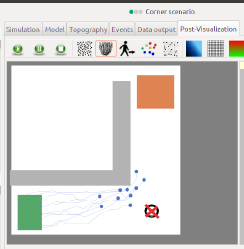
\includegraphics[width=\textwidth]{images/task3(goal).png}
    \caption{Setup of the scenario}
    \label{fig: 3a}
 \end{subfigure}
 \begin{subfigure}[b]{0.4\textwidth}
      \centering
     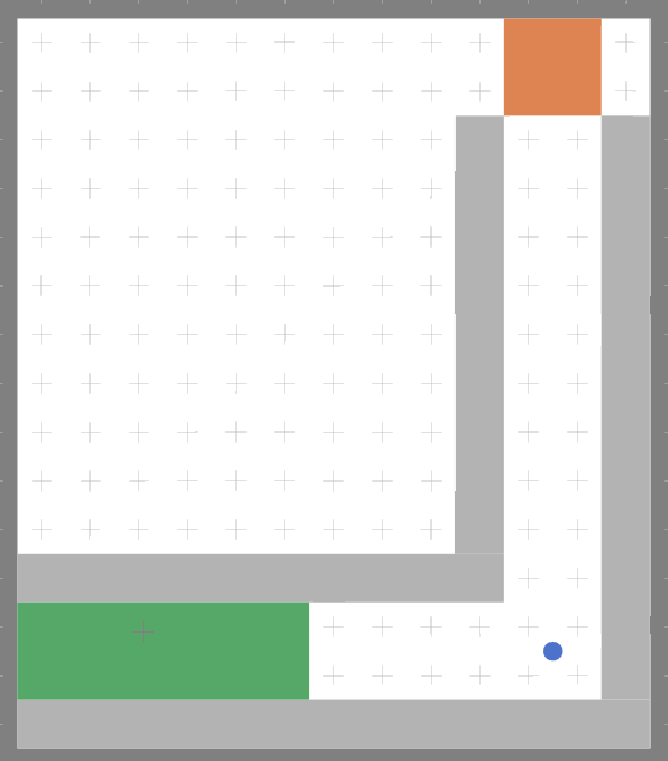
\includegraphics[width=\textwidth]{images/task3(done).png}
     \caption{New pedestrian placement}
     \label{fig: 3b}
 \end{subfigure}
 \end{figure}


In our simulation task, we introduced a new pedestrian into the scenario. The addition of this new pedestrian, positioned closer to the target, would cause different outputs of the scenario. The scenario output results minorly differed in \texttt{overlaps.csv}, particularly 'distance-PID3' and 'overlaps-PID3'. We could observe that the first ones to arrive were the added pedestrians that took 9 seconds to get to the target, due to their closer proximity. The last ones of the pedestrians originated from the standard starting point and took 30.293 seconds to reach the target. This outcome was achieved by the OSM model.